\documentclass[bare_jrnl_transmag]{subfiles}
\begin{document}

\subsection{Vision Assessment}
The error in the relative transformation output from the vision system was measured across 500 dataset samples. Errors were quantified as the difference between measured and ground-truth transformations in the drone reference frame. Translational errors were computed as vector differences. Rotational errors were represented in Rodriguez vector form. Results are shown in Table \ref{tab:vision-error-stats}.

\begin{table}[H]
    \centering
    \begin{tabular}{lccc}
    \hline
    Axis & Mean error [m] & Variance [m] & RMS error [m] \\ \hline
    $x$ & -0.0146 & 0.0226 & 0.1510 \\
    $y$ & -0.0406 & 0.0175 & 0.1383 \\
    $z$ & -0.0040 & 0.0068 & 0.0826 \\ \hline
    Axis & Mean error [rad] & Variance [rad] & RMS error [rad] \\ \hline
    $\theta_x$ & -0.0080 & 0.0015 & 0.0397 \\
    $\theta_y$ & -0.0071 & 0.0005 & 0.0234 \\
    $\theta_z$ & 0.0166 & 0.0013 & 0.0394 \\ \hline
    \end{tabular}
    \label{tab:vision-error-stats}
\end{table}

\begin{figure}[H]
    \centering
    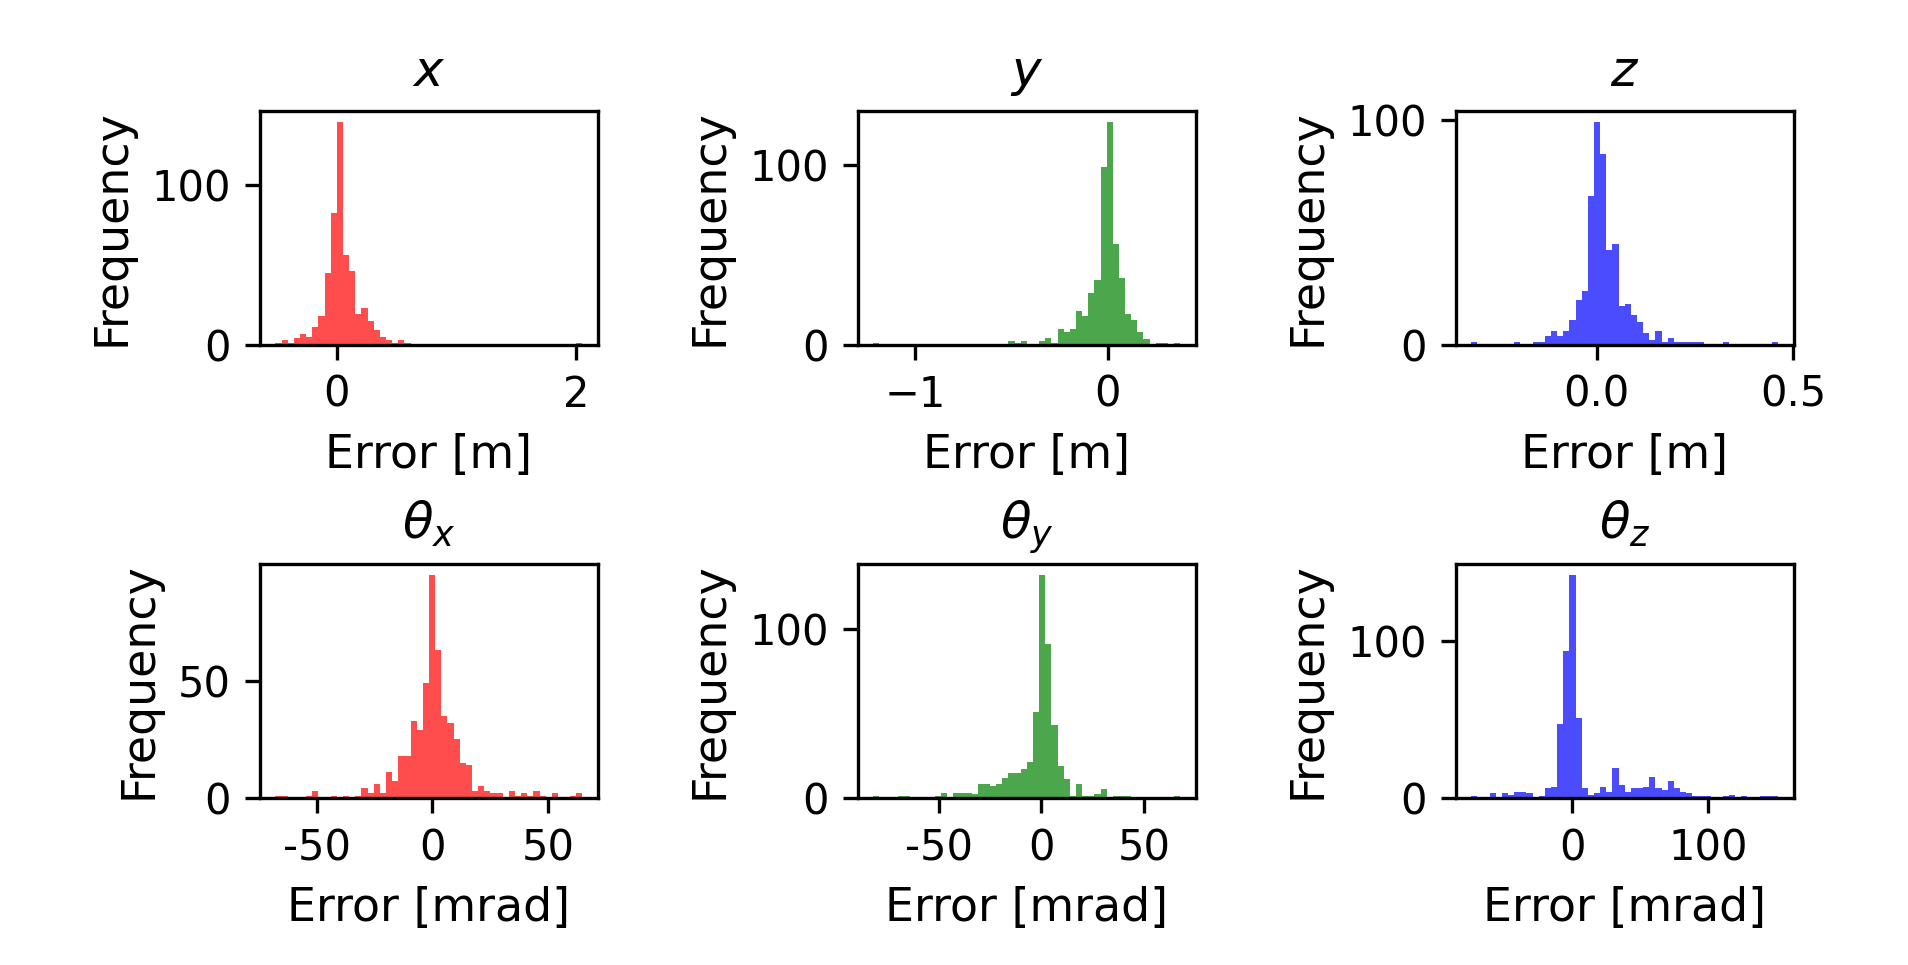
\includegraphics[width=0.9\linewidth]{figures/vision_error.png}
    \caption{Distribution of error components in relative vision odometry output. Measured across 500 samples of the dataset.}
    \label{fig:vision-error-results}
\end{figure}

\end{document}